\documentclass[11pt]{article}
\usepackage{amsmath, amssymb, amsfonts,  graphicx, enumerate, float, wrapfig}
\usepackage[margin=0.5in]{geometry}
\graphicspath{{./}}
\newcommand*{\vs}{\vspace{1cm}}
\newcommand*{\next}{\noindent}
\newcommand*{\set}{\setcounter{equation}{0}}


\title{Notes - 3.7 Optimization Problems}
\author{Juan J. Moreno Santos}
\date{October 2023}

\begin{document}
\maketitle

\section{Warm-up}
1. An equation of the line tangent to the graph of $f(x)=x(1-2x)^3$ at the point (1, -1) is\\
Expanding this quartic results in the following simplification:
\begin{align}
    a^3+3a^2b+3ab^2+b^3\\
    1^3+3(1)^-2x+3(1)^1-(-2x)^2+(-2x)^3\\
    1-6x+12x^2-8x^3\\
    x-6x^2+12x^3-8x^4\\
\end{align}
Therefore,
\begin{align}
    y+7=-7(x-1)\\
    y+1=-7x+7\\
    y=-7x+6\\
\end{align}
Using the product rule,
\begin{align}
    \set
    f'(x)&=1(1-2x)^3+x3(1-2x)^2(-2)\\
    &=(1-2x^3)-6x(1-2x)^2\\
    &=-1-6=-7=m
\end{align}
Refer to equation 6.

\section{Reminder about limits}
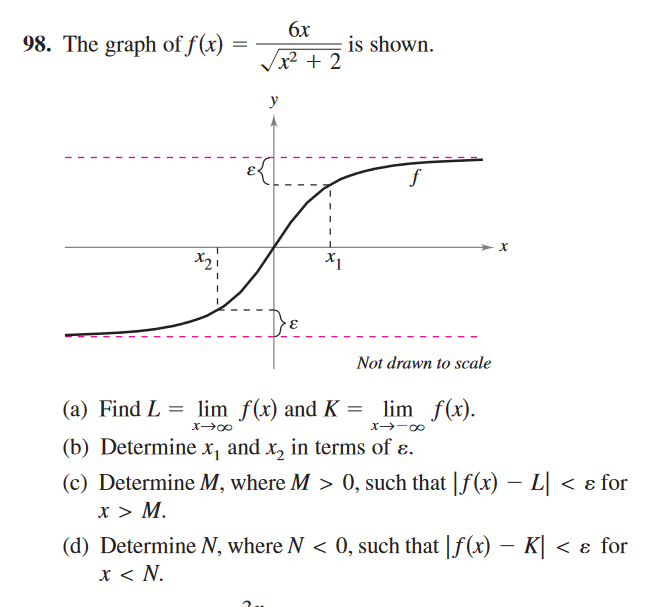
\includegraphics{firefox_H3E8UqRM15.png}\\
Remember that $|x|=\sqrt[]{x^2}$.\\
Dividing coefficients will produce both a negative and a positive asymptote, so the limits approach different values from both sides.
\section{The box problem}
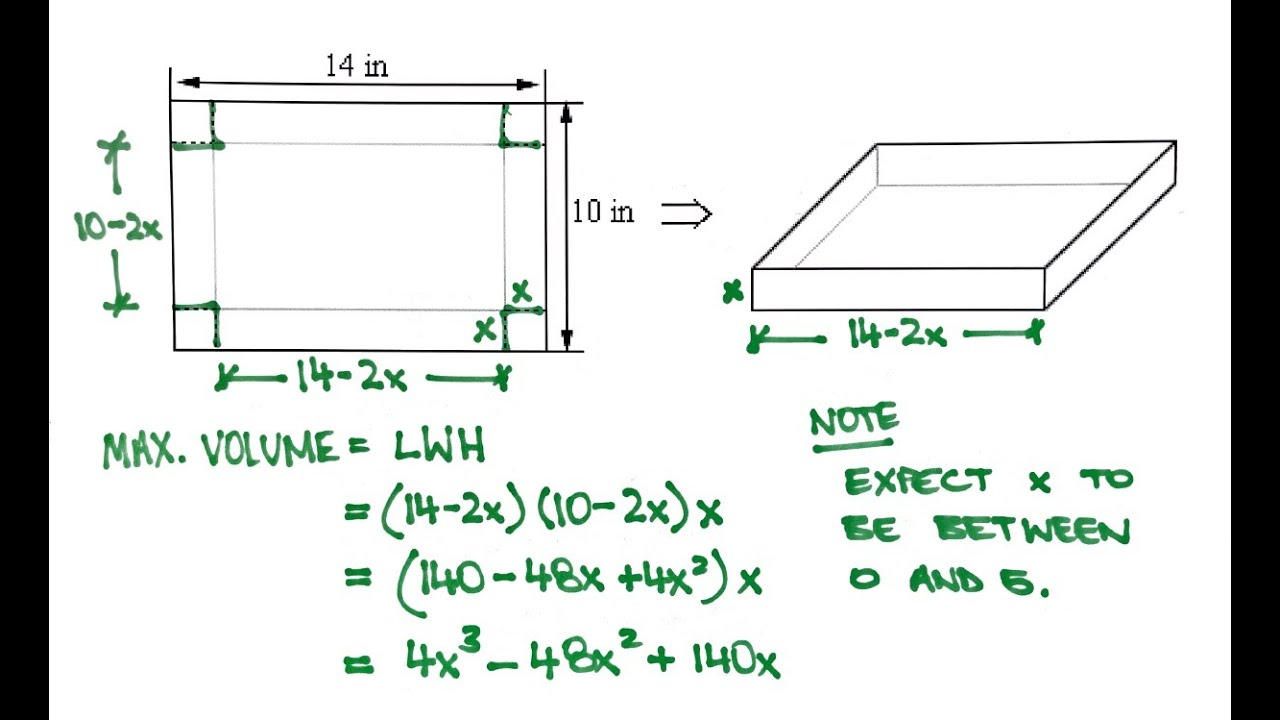
\includegraphics[scale=0.25]{maxresdefault.jpg}
\section{Find two positive numbers that satisfy the given requirements}
5. The product is 147 and the sum of the first number plus three times the second number is a minimum.
\begin{align}
    \set
    xy=147\\
    y=\frac{147}{x}
\end{align}
\begin{align}
    x+3y= minimum\\
    (x+3)(\frac{147}{x})= minimum\\
    minimum'=1-\frac{3\cdot 147}{x^2}=0\\
    1=\frac{3\cdot 147}{x^2}\\
    x^2=3.147\therefore\,\,\,\, x=21,\,\,\,\, y=7\\
\end{align}

\section{Find the length and width of a rectangle that has the given perimeter and a maximum area.}
10. Perimeter: $P$ units
\begin{align}
    \set
    Area_{max}=A_{max}&=xy\\
    Perimeter=P&=2x+2y\\
    \frac{P-2x}{2}&=y\\
    A{max}&=x\left(\frac{p-2x}{2}\right)\\
    &=\frac{1}{2}Px-x^2\\
    A'=\frac{P}{2}-2x=0\,\,\text{when}\,\, x=\frac{P}{4},\,\,\,\, y=\frac{P}{4}
\end{align}

\section{11/02/2023 Warm-up}
1.\begin{align}
    \set
    f(x)&=\sqrt[]{2x}\\
    f'(1)&=\frac{1}{\sqrt[]{2x}}\\
    &=\frac{1}{\sqrt[]{2\cdot 1}}(\frac{\sqrt[]{2}}{\sqrt[]{2}})\\
    &=\frac{\sqrt[]{2}}{2}
\end{align}

2.\begin{align}
    \set
    f(x)&=\frac{x^2+1}{x},\,\,\,\, g(x)=4x+7\\
    h(x)&=f(x)\cdot g(x)\\
    h'(x)&=f'(x)g(x)+f(x)g'(x)\\
    h'(x)&=(1-x^-2)(4x+7)+(x+\frac{1}{x})(4)\\
    h'(1)&=8,\,\,\,\, f(1)=0,\,\,\,\, g'(1)=4
\end{align}

\section{3.7 P-set example problems}
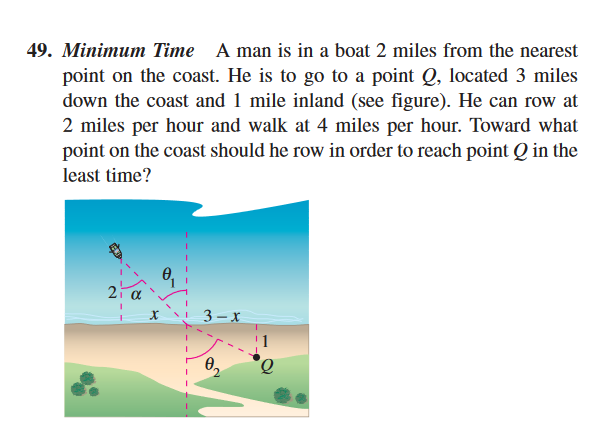
\includegraphics{49.png}
\begin{align}
    \set
    Distance=rate_1time_1+rate_2time_2=D=r_1t+r_2t\\
\end{align}

\vs
\next
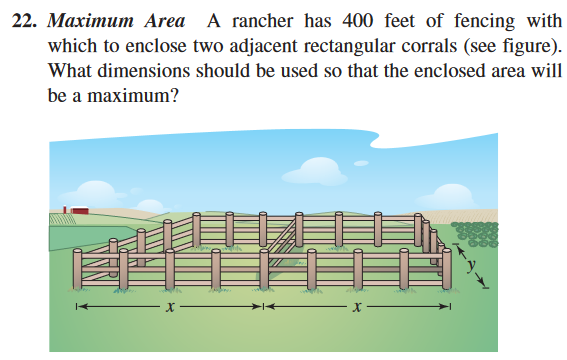
\includegraphics{22.png}
\begin{align}
    \set
    400ft&=4x+3y\\
    x&=\frac{400-3y}{4}\\
    Area=A&=2x\cdot y\\
    &=2\left(\frac{400-3y}{4}\right)y\\
    &=200y-\frac{3}{2}y^2\\
    A'&=200-3y=0
    y=\frac{200}{3}
\end{align}
Solving for x:
\begin{align}
    400&=3\left(\frac{200}{3}\right)+4x\\
    200&=4x\\
    50&=x
\end{align}
Since the fence is $2x$, the dimensions of the enclosed area will be 100ft by $\frac{200}{3}$ft.






\end{document}